1;95;0c

\documentclass[letterpaper,aps,prl,superscriptaddress,floatfix,twocolumn]{revtex4}

\usepackage{graphicx}
%\usepackage[scientific-notation=true]{siunitx}
\usepackage{amsmath}
\usepackage{amssymb}
\usepackage{booktabs}
\usepackage{rotating}
\usepackage[]{units}
%\usepackage{caption}
\graphicspath{ {./Analysis-Primer/Primer_Images/} }

\begin{document}

\title{MARATHON Pass 2 Analysis Primer}

\author{Jason Bane}
\author{Tyler Hague}
\author{Tyler Kutz}
\author{Hanjie Liu}
\author{Mike Nycz}
\author{Tong Su}

\author{Evan McClellan}
%\affiliation{Thomas Jefferson National Accelerator Facility}


\date{\today}

\begin{abstract}
\end{abstract}

\maketitle

\section{I. Overview}

\section{II. Replay}
 (Tyler Hague)

\section{III. Calibrations}

 \subsection{i. E/p}
 (Mike Nycz)

 \subsection{ii. VDC}

 \subsection{iii. Raster}
 (Tyler Hague)

 \subsection{iv. BCM}
\subsection{Unser and Beam Current Monitors Calibration}
In order to accurately calibrate the BCM's, first the unser must be calibrated. The unser is used as an absolute reference to which the BCM's are calibrated to. The procedure to calibrate the unser involves sending a constant and known currents through a thin wire inside of the unser. A series of currents with, over a range between 2.5 - 100 $\mu$A,during 90 second intervals, as can be seen in figure (??). which shows the frequency response of the unser for the various currents. A linear fit of sent current vs the unser response, determines an overall gain factor for the unser. The gain of the unser of calibrated 4 times during MARATHON before each BCM calibration was preformed, in order to check the unser's stability. Figure(??) shows the unser was stable during the entirety of the MARATHON run. 

\begin{table}[ht]
\caption{Unser Calibration Results}
%\centering
\begin{center}
\begin{tabular}{l| c| c| c| r}
Date & 03-05 & 03-28 & 4-03 & 04-06  \\
\hline
Unser Gain & 2.526e-4 & 2.524e-4 & 2.529e-4 & 2.527e-4\\
\end{tabular}
\end{center}
\end{table}

Having calibrated the unser, we can then calibrate the BCMs in a similar manner to the calibration of the unser but replacing the current from a wire with current from the electron beam. For the BCM calibrations during MARATHON and all Tritium experiments, the range in current was between 3 - 22.5 $\mu$A. Again, the procedure intervals of 90 seconds (i.e 90 seconds of continuous current to the Hall followed by 90 seconds with no beam). 
The Calibration procedure requires making cuts in the frequency response of the unser and BCM receiver and integrating the total amount of frequency to determine the average frequency of the receiver during the given time interval. An example of the cuts made is shown in figure 3

The unser frequency during the calibration can be related to the delivered current using the gain factor determined from the unser calibration. 
\begin{equation}
I_{unser} = gain * f_{unser}
\end{equation}

By then plotting $I_{unser} vs freq_{BCM}$ and fitting with a linear function, the gain and offset (which are proportional the slope and intercept of the fit respectively) of each BCM receiver can be determined. The gain 



%unser
\begin{figure}[H]
\begin{center}
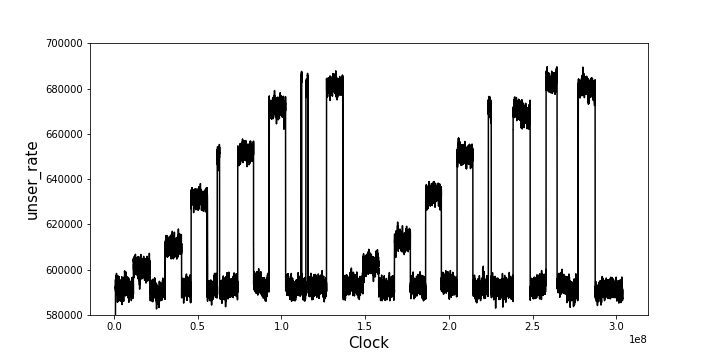
\includegraphics[angle=0, scale =0.65]{Unser_freq.png}
\end{center}
\caption{BCM Calibration : unser}
\end{figure}
%dnew
\begin{figure}[H]
\begin{center}
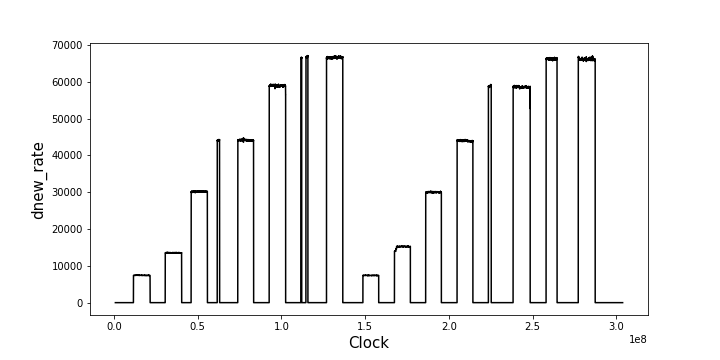
\includegraphics[angle=0, scale =0.65]{Dnew_freq.png}
\end{center}
\caption{BCM Calibration : dnew}
\end{figure}


\begin{figure}[H]
\begin{center}
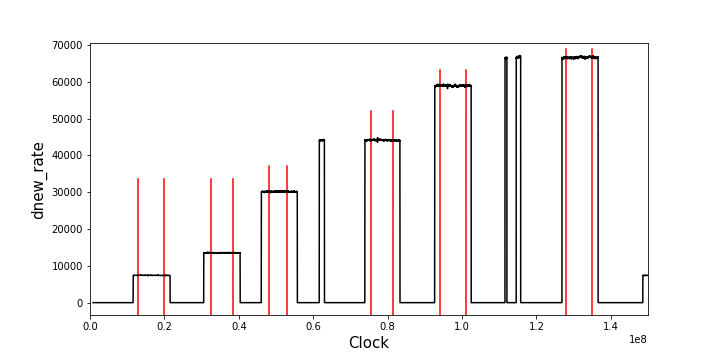
\includegraphics[angle=0, scale =0.65]{Dnew_freq_cuts.png}
\end{center}
\caption{Frequency cuts}
\end{figure}

Table(??) shows the result of the 3 BCM calibrations for the dnew digital BCM receiver.
\begin{table}[ht]
\caption{BCM Calibration Results}
%\centering
\begin{center}
\begin{tabular}{l| c| c| r}
   & 03-05 & 03-28 & 4-03 \\
\hline
dnew Gain & 3.3358e-4 & 3.3351e-4 & 3.3372e-4\\
\hline
dnew offset & -0.097  &   0.003   & 0.132         \\
\end{tabular}
\end{center}
\end{table}


 \subsection{v. BPM}
\subsection{BPM PreBeam Check}



 

 \subsection{vi. Optics}

\section{IV. Corrections}

 \subsection{i. PID}

 \subsection{i. Positron Subtraction}
 (Tong Su)

 \subsection{ii. Endcap Subtraction}
 (Tong Su)

 \subsection{iii. Livetime}

 \subsection{iv. Tritium Decay}
 \subsection{Target composition}

Tritium decays to helium via the $\beta$-decay process $^3\text{H} \,\rightarrow\, ^3\text{He} + e^- + \overline{\nu}_e$, with a half-life of

\begin{equation*}
\tau_{1/2} = \ln(2)\tau = (4500 \pm 8) \text{ days} 
\end{equation*}

This results in a time-dependent target composition, with a decreasing (increasing) population of tritium (helium) nuclei.  These effects must be quantified and corrected in order to accurately extract the normalized tritium yield from tritium target data.

The target cell was filled with an initial tritium number density $n_T^0$, and initial helium number density $n_H^0$.  As tritium decays to helium, these number densities evolve in time as
\begin{align}
n_T &= n_T^0 \: e^{-t/\tau} \label{nT}\\[5pt]
n_H &= n_H^0(1 - e^{-t/\tau}) \label{nH},
\end{align}
where $t$ is the number of days since the target was filled.  Since the decay process preserves the total number of nuclei, the total number density $n_{tot}$ is constant in time:
\begin{align}
n_{tot} 	&= n_T + n_H \nonumber \\
		&= n_T^0 + n_H^0 
\end{align} 

With these quantities, the helium fraction can be defined:
\begin{equation}
f_H = \frac{n_H}{n_T + n_H} = \frac{n_H}{n_{tot}} \label{fH}
\end{equation}
Given an infinite amount of time, all of the tritium will decay to helium.  Therefore $f_H\rightarrow1$ as $t\rightarrow\infty$.  

\subsection{Normalized yield correction}

The normalized yield is defined as:
\begin{equation}
Y = \frac{N}{Qn},
\end{equation}
where $N$ is the number of detected electrons, $Q$ is the beam charge incident on the target, and $n$ is the target number density.  Assume that $N$ includes all corrections (deadtime, efficiency, endcap contamination, etc.) \textit{not} related to tritium decay.  In practice, the yield is extracted from multiple runs, so the number of detected electrons and luminosity must be summed over run number $i$:
\begin{equation}
Y = \frac{\sum N_i}{\sum Q_i n_i},
\end{equation}

The required correction must account not only for the evolution of the target composition (quantified in the previous section), but also for the fact that some of the detected electrons $N$ will have actually scattered from a helium nucleus instead of a tritium nucleus.  Begin by expressing the raw, uncorrected normalized yield (which is measured) as

\begin{equation}
Y_{raw} = \frac{\sum (T_i + H_i)}{\sum Q_i (n_{T,i} + n_{H,i})} \label{Yraw}
\end{equation}
where $T$ and $H$ are the number of detected electrons scattered by tritium and helium, respectively.  For time-dependent quantities (such as $n_{T,i}$ and $n_{H,i}$, given by Equations \ref{nT} and \ref{nH}), the subscript indicates the value of the quantity at the time of run $i$.  The goal is to obtain the normalized tritium yield $Y_T$ in terms of $Y_{raw}$ and correction factors, where

\begin{equation}
Y_T = \frac{\sum T_i}{\sum Q_i n_{T,i}}. 
\end{equation} 

Due to the helium contamination, the correction factor will depend on the normalized helium yield

\begin{equation}
Y_H = \frac{\sum H_i}{\sum Q_i n_{H,i}}. 
\end{equation}

From equation (\ref{Yraw}), only a few steps of algebra are required to obtain $Y_T$.  Recall that the total number density $n_{tot}=n_T + n_H$ is constant in time, and note that the tritium fraction $n_{T,i}/n = 1 - f_{H,i}$, where $f_H$ is the helium fraction defined by Equation \ref{fH}.

\begin{align*}
Y_{raw} 	&= \frac{\sum (T_i + H_i)}{\sum Q_i (n_{T,i} + n_{H,i})} \\[15pt]
		&= \frac{\sum T_i}{n_{tot} \sum Q_i} + \frac{\sum H_i}{n_{tot} \sum Q_i} \\[15pt]
		&= \left(\frac{\sum_i T_i}{\sum_i Q_i n_{T,i}}\right)\left(\frac{\sum_i Q_i n_{T,i}}{n_{tot} \sum_i Q_i}\right)
		+ \left(\frac{\sum_i H_i}{\sum_i Q_i n_{H,i}}\right)\left(\frac{\sum_i Q_i n_{H,i}}{n_{tot} \sum_i Q_i}\right) \\[15pt]
		&= Y_T\left(\frac{\sum Q_i(1-f_{H,i})}{\sum Q_i}\right) + Y_H\left(\frac{\sum Q_i f_{H,i}}{\sum Q_i}\right)
\end{align*}

To simplify notation, define the charge-averaged helium fraction:

\begin{equation}
\langle f_H \rangle \equiv \frac{\sum Q_i f_{H,i}}{\sum Q_i}
\end{equation}

Thus,

\begin{equation}
Y_{raw} = Y_T(1-\langle f_H \rangle) + Y_H \langle f_H \rangle,
\end{equation}

and finally,

\begin{equation}
Y_T = Y_{raw}\left(\frac{1}{1-\langle f_H \rangle}\right) - Y_H \left(\frac{\langle f_H \rangle}{1-\langle f_H \rangle}\right)
\end{equation}

\subsection{Uncertainty propagation}

Pending



 \subsection{v. Boiling}
 (Tong, Mike)

 \subsection{vi. Radiative Corrections}
 (Hanjie Liu)

\section{V. Binning and Combining}

 \subsection{Bin width Choice}

 \subsection{Bin Centering}

 \subsection{Combining Kinematic Overlap}

\end{document}

